% ============================================================
% main.tex — Assignment 2, Part 2: Secure Computing
% Compile in Overleaf with pdfLaTeX.
% Run sequence: pdfLaTeX → BibTeX → pdfLaTeX → pdfLaTeX
% ============================================================
\documentclass[12pt,a4paper]{article}

% ---- Encoding & font ----
\usepackage[T1]{fontenc}
\usepackage[utf8]{inputenc}
\usepackage{lmodern}
\usepackage{microtype}

% ---- Page geometry ----
\usepackage[top=2.5cm,bottom=2.5cm,left=2.5cm,right=2.5cm]{geometry}

% ---- Math ----
\usepackage{amsmath}

% ---- Graphics ----
\usepackage{graphicx}

% ---- TikZ (pipeline diagram) ----
\usepackage{tikz}
\usetikzlibrary{arrows.meta, shapes.geometric, positioning, fit, backgrounds, calc}

% ---- Tables ----
\usepackage{booktabs}
\usepackage{array}
\usepackage{tabularx}
\usepackage{multirow}
\usepackage{longtable}
\usepackage{colortbl}

% ---- Spacing & lists ----
\usepackage{setspace}
\usepackage{enumitem}
\setlist[itemize]{leftmargin=1.5em, itemsep=2pt, topsep=4pt}
\setlist[enumerate]{leftmargin=1.5em, itemsep=2pt, topsep=4pt}

% Paragraph spacing (TinyTeX-friendly replacement for parskip package)
\setlength{\parindent}{0pt}
\setlength{\parskip}{6pt}

% ---- Headers & footers ----
\usepackage{fancyhdr}
\usepackage{lastpage}

% ---- Colours ----
\usepackage[dvipsnames, table]{xcolor}
\definecolor{phaseblue}{RGB}{31,90,160}
\definecolor{cplan}{RGB}{142,68,173}
\definecolor{ccode}{RGB}{41,128,185}
\definecolor{cbuild}{RGB}{39,174,96}
\definecolor{ctest}{RGB}{230,126,34}
\definecolor{crelease}{RGB}{192,57,43}
\definecolor{cdeploy}{RGB}{22,160,133}
\definecolor{cmonitor}{RGB}{52,73,94}
\definecolor{lightgray}{RGB}{245,245,245}
\definecolor{screengray}{RGB}{220,220,220}
\definecolor{highred}{RGB}{214,39,40}
\definecolor{medorange}{RGB}{255,127,14}
\definecolor{lowgreen}{RGB}{44,160,44}

% ---- Hyperlinks ----
\usepackage[colorlinks=true, linkcolor=phaseblue, citecolor=phaseblue,
            urlcolor=phaseblue, bookmarks=true]{hyperref}

% ---- Code listings ----
\usepackage{listings}
\lstset{
  basicstyle=\ttfamily\footnotesize,
  breaklines=true, frame=single,
  backgroundcolor=\color{lightgray},
  keywordstyle=\color{blue}\bfseries,
  commentstyle=\color{green!55!black},
  stringstyle=\color{red!70},
  numbers=left, numberstyle=\tiny\color{gray!60},
  numbersep=6pt, xleftmargin=12pt
}

% ---- Boxes ----
\usepackage{framed}
\setlength{\FrameSep}{6pt}
\setlength{\FrameRule}{0.6pt}

\newenvironment{secbox}[1]{%
  \begin{framed}
  \noindent\textbf{\color{phaseblue}#1}\par\medskip
}{%
  \end{framed}
}

\newenvironment{warnbox}[1]{%
  \begin{framed}
  \noindent#1\par\medskip
}{%
  \end{framed}
}

\newenvironment{notebox}{%
  \begin{framed}
  \noindent
}{%
  \end{framed}
}

% ---- Float control ----
\usepackage{float}
\usepackage{caption}
\usepackage{subcaption}
\captionsetup{font=small, labelfont=bf}

% ---- Landscape pages ----
% Rotate landscape pages in the PDF output so they are readable without manual rotation.
\usepackage[pdftex]{lscape}

% ---- Bibliography ----
\usepackage[authoryear,round,sort&compress]{natbib}
\bibliographystyle{apalike}

% ---- Section formatting ----
\usepackage{titlesec}
\titleformat{\section}
  {\Large\bfseries\color{phaseblue}}
  {Question \thesection:}{0.6em}{}
  [\vspace{-4pt}\textcolor{phaseblue}{\rule{\linewidth}{0.8pt}}]
\titleformat{\subsection}{\normalsize\bfseries\color{phaseblue!80!black}}{\thesubsection}{0.5em}{}
\titleformat{\subsubsection}{\normalsize\bfseries}{}{0em}{}

% ---- Page style ----
\pagestyle{fancy}
\setlength{\headheight}{14pt}
\fancyhf{}
\lhead{\small\textit{Secure Computing --- Assignment 2, Part 2}}
\rhead{\small\textit{DevSecOps \& Application Security}}
\cfoot{\small Page \thepage\ of \pageref{LastPage}}
\renewcommand{\headrulewidth}{0.4pt}

% ---- Misc ----
\usepackage{rotating}
\usepackage{pifont}
\newcommand{\cmark}{\textcolor{lowgreen}{\ding{51}}}
\newcommand{\xmark}{\textcolor{highred}{\ding{55}}}

% Screenshot placeholder command
\newcommand{\screenshot}[2][8cm]{%
  \begin{center}
  \fcolorbox{gray!60}{screengray!40}{%
    \begin{minipage}{0.92\textwidth}
    \centering
    \vspace{0.9cm}
    {\small\textit{\textbf{[SCREENSHOT PLACEHOLDER]}}\\[4pt]#2}
    \vspace{0.9cm}
    \end{minipage}
  }
  \end{center}
}

% ============================================================
\begin{document}
\onehalfspacing

% ============================================================
% TITLE PAGE
% ============================================================
\begin{titlepage}
  \centering
  \vspace*{1.5cm}
  {\color{phaseblue}\rule{\linewidth}{1.5pt}}\\[0.6em]
  {\Huge\bfseries\color{phaseblue} Secure Computing\\[0.3em]}
  {\Large\bfseries Assignment 2 --- Part 2\\[0.5em]}
  {\color{phaseblue}\rule{\linewidth}{1.5pt}}\\[2.5cm]

  {\large DevSecOps, Threat Modelling,\\[0.2em]
   Vulnerability Assessment \& Supply Chain Security}\\[3cm]

  \begin{tabular}{@{}ll@{}}
    \textbf{Student:}     & Dylan Walt \\[0.4em]
    \textbf{Student No.:} & 2726341 \\[0.4em]
    \textbf{Module:}      & Secure Computing \\[0.4em]
    \textbf{Assessment:}  & Assignment 2 --- Part 2 \\[0.4em]
    \textbf{Year Level:}  & Fourth Year, Semester 1 \\[0.4em]
    \textbf{Date:}        & \today \\
  \end{tabular}

  \vfill
  {\small Submitted in partial fulfilment of the requirements for the module on Secure Computing.}
\end{titlepage}

% ---- Table of Contents ----
\newpage
\tableofcontents
\newpage

% ============================================================
% QUESTION 1 — DevSecOps Critical Evaluation (20 marks)
% ============================================================
\section{DevSecOps Critical Evaluation}

\begin{secbox}{Assessment Requirement}
Critically evaluate the effectiveness of DevSecOps in reducing modern application security risks.
Maximum: 1\,200 words.
\end{secbox}

\vspace{0.5em}

\subsection*{Introduction}

DevSecOps represents a maturation of the DevOps model, embedding security as a shared
responsibility across development, security, and operations teams throughout the entire
software delivery lifecycle (SDL). Despite increasing adoption of CI/CD pipelines and
automated security tooling, organisations continue to suffer significant security breaches.
The 2021 Log4Shell vulnerability and the 2020 SolarWinds supply chain compromise
illustrate that technical tooling alone is insufficient. This essay critically evaluates
DevSecOps effectiveness across six dimensions: Shift Left Security, the limitations of
automation, organisational culture, false positives and tool overload, open-source
dependency risk, and the necessity of continuous monitoring.

\subsection*{Shift Left Security}

``Shifting Left'' denotes the practice of integrating security review, testing, and
architectural analysis earlier in the SDL, reducing the cost and consequence of
vulnerability discovery. Research by \citet{ibm2012} demonstrated that a defect identified
at the design phase costs up to 30 times less to remediate than one discovered in
production. In practice, Shift Left manifests through embedding Static Application Security
Testing (SAST) tools such as SonarLint directly into developer IDEs, conducting threat
modelling exercises during sprint planning using frameworks such as STRIDE or PASTA, and
enforcing security-focused pull request review policies. Microsoft's Security Development
Lifecycle (SDL) is a canonical example: by mandating threat modelling, static analysis, and
security sign-off at every development milestone, Microsoft demonstrably reduced the
vulnerability density of its products \citep{howard2006}. However, Shift Left Security is
effective only when developers receive adequate security training and when tooling generates
actionable, low-noise guidance. Without security awareness education, Shift Left degrades
into a series of automated gates that developers learn to suppress rather than remediate,
undermining the very premise of the approach \citep{johnson2013}.

\subsection*{Why Automation Alone is Insufficient}

Automated security tooling accelerates vulnerability discovery at scale, yet it carries
well-documented limitations that preclude it from replacing human judgement. SAST tools
operate on predefined rule sets and are unable to detect logical business-logic
vulnerabilities, authentication flaws rooted in contextual misuse, or race conditions that
require semantic understanding of application behaviour \citep{livshits2005}. The 2020
SolarWinds SUNBURST supply chain attack is emblematic of automation's blind spots:
malicious code was surgically inserted into a trusted build pipeline at a stage where
automated scanners classified the output as a legitimate, signed artefact
\citep{cisasolarwinds2021}. No static or dynamic scanner triggered an alert because the
attack exploited the trustworthiness of the pipeline itself. Similarly, Dynamic Application
Security Testing (DAST) tools cannot replicate the creative, context-driven reasoning of a
skilled penetration tester exploring novel attack chains. The \citet{nist2018} Cybersecurity
Framework explicitly positions automated detection controls within a broader,
human-governed risk management programme, emphasising that automation must augment
security professionals rather than supplant them.

\subsection*{The Importance of Organisational Culture}

Before it is a technical transformation, DevSecOps is a cultural one. Effective
implementation requires dismantling the traditional model in which a siloed security
function gates software releases, replacing it with a shared-ownership model in which every
team member bears proportionate security responsibility \citep{kim2016}.
\citet{forsgren2018} demonstrated through large-scale empirical research that
high-performing software organisations exhibit generative cultures characterised by
psychological safety, high cooperation, and blameless post-incident reviews --- cultural
properties that are prerequisite for sustainable security improvement. Organisations that
deploy DevSecOps tooling without corresponding cultural alignment frequently encounter
developer resistance, security team marginalisation, and chronic under-investment in
security skills development. The 2019 Capital One breach, in which a misconfigured AWS Web
Application Firewall enabled a server-side request forgery (SSRF) attack resulting in the
exfiltration of over 100 million customer records, reflected not merely a technical failure
but an organisational failure in cloud configuration governance, access management review,
and security accountability structures \citep{senate2019}.

\subsection*{Challenges of False Positives and Tool Overload}

A persistent operational challenge in DevSecOps adoption is the generation of excessive
false positive alerts by automated security tools. \citet{johnson2013} found that a primary
reason developers dismiss static analysis results is the perceived inaccuracy of tool
output, with false positive rates exceeding 50\% in large enterprise codebases. When the
signal-to-noise ratio of a security tool is poor, development teams rationally develop
alert fatigue, increasing the probability that genuine vulnerabilities are dismissed
alongside spurious warnings. Compounding this, organisations frequently adopt multiple
overlapping security tools simultaneously --- SAST, DAST, Software Composition Analysis
(SCA), container image scanning, infrastructure-as-code scanning, and secret detection ---
without centralised orchestration. The resulting fragmented security landscape makes
triaging, prioritising, and tracking vulnerabilities operationally unmanageable, leading to
security debt accumulation rather than reduction. Platforms such as DefectDojo can
consolidate findings, but organisations still need deliberate tool rationalisation, clear
remediation SLAs, and executive accountability; otherwise low-confidence alerts obscure
actionable risk.

\subsection*{The Impact of Vulnerable Open-Source Dependencies}

Modern applications are substantially composed of open-source libraries, creating systemic
software supply chain risk. The 2021 Log4Shell vulnerability (CVE-2021-44228) in the
widely-deployed Apache Log4j logging library exposed an estimated three billion devices
globally and required emergency cross-industry patching at unprecedented scale
\citep{chen2022}. The 2017 Equifax data breach similarly exploited CVE-2017-5638, a
critical known vulnerability in the Apache Struts web framework that had remained unpatched
for approximately two months due to inadequate dependency lifecycle management, ultimately
exposing the personal and financial data of 147 million consumers \citep{ftc2019}. SCA
tools such as OWASP Dependency-Check, Snyk, and GitHub Dependabot provide automated
identification of known vulnerabilities by querying the National Vulnerability Database
(NVD) and the GitHub Advisory Database. However, SCA is inherently reactive, detecting
established CVEs while remaining blind to zero-day vulnerabilities and deliberately
malicious packages, as demonstrated by the 2021 compromise of the \texttt{ua-parser-js}
npm package. Organisations must therefore complement automated SCA with Software Bill of
Materials (SBOM) generation per NTIA guidance \citep{ntia2021sbom}, dependency version
pinning, and supply chain security assessments.

\subsection*{Why Continuous Monitoring Remains Necessary After Deployment}

Deploying an application does not conclude the security lifecycle. Post-production threats
including runtime exploits, newly disclosed zero-day vulnerabilities, insider threats, and
advanced persistent threats (APTs) necessitate continuous monitoring capabilities
independent of the pre-deployment pipeline. The inadequacy of deployment-gate security is
starkly demonstrated by the Equifax breach, in which attackers exfiltrated data for 78 days
before detection \citep{ftc2019}, and by the 2013 Target breach, in which security
monitoring tools generated alerts that were not acted upon by operations staff. Tools such
as Falco for container runtime security, AWS GuardDuty for cloud-native threat detection,
and SIEM platforms such as Splunk or Elastic Security provide real-time production
visibility. \citet{nist800137} mandates Information Security Continuous Monitoring (ISCM)
as a fundamental governance requirement, emphasising that threat landscapes evolve
independently of the software delivery cycle. Effective DevSecOps programmes treat
continuous monitoring as an integral pipeline stage, with defined alerting thresholds,
automated incident response runbooks, and feedback loops that propagate production findings
upstream into backlog prioritisation and threat model updates. Quantitatively,
\citet{forsgren2018} found that elite software delivery organisations restore service from
failures 2,604 times faster than low-performing counterparts --- an outcome achievable only
through comprehensive observability and rapid-response monitoring. This underscores that
continuous monitoring is not merely a reactive security control but a strategic organisational
capability that enables evidence-based improvement and informed risk governance.

\subsection*{Conclusion}

DevSecOps can materially reduce application security risk by embedding security controls
throughout the software delivery lifecycle, but only when supported by cultural change,
informed human review, and continuous monitoring. Treating DevSecOps as a tooling
procurement exercise leaves organisations exposed; sustained improvement requires
accountable ownership, prioritised remediation, and feedback loops that keep pace with
evolving threats.

\vspace{0.5em}
\begin{notebox}
\textit{Approximate word count: 1\,165 words}
\end{notebox}

\newpage

% ============================================================
% QUESTION 2 — PayWave Digital DevSecOps Pipeline (30 marks)
% ============================================================
\section{Scenario-Based Design: PayWave Digital DevSecOps Pipeline}

\begin{secbox}{Scenario Summary}
PayWave Digital is a Johannesburg-based FinTech startup launching a cloud-native digital
payments platform (microservices, Docker, AWS, GitHub Actions). Key risks identified during
due-diligence: vulnerable OSS dependencies, secrets committed to GitHub, absent automated
security testing, and insufficient runtime monitoring.
\end{secbox}

\subsection{Security Risk Analysis}

Before designing the DevSecOps pipeline, a structured analysis of PayWave's identified
risks is essential:

\begin{enumerate}
  \item \textbf{Vulnerable open-source dependencies.} Heavy reliance on open-source
    libraries for authentication, logging, payment processing, and API management creates
    a broad attack surface. Libraries may contain known CVEs and are typically not
    audited before inclusion \citep{snyk2023}.

  \item \textbf{Secrets management failures.} A developer accidentally committed live
    API credentials to a private GitHub repository. Without automated secret detection
    and centralised secrets management, credentials may persist in version history and
    propagate across environments.

  \item \textbf{Absent automated security testing.} No SAST, DAST, or SCA tooling is
    integrated into the GitHub Actions pipeline. Vulnerabilities are not discovered until
    after deployment or, worse, after exploitation.

  \item \textbf{Insufficient runtime monitoring.} Without real-time production
    monitoring, the team cannot detect anomalous API access patterns, container escapes,
    data exfiltration, or fraud-related anomalies indicative of active compromise.

  \item \textbf{Container and infrastructure risks.} Docker containers without image
    scanning may run with known OS-level or library-level vulnerabilities. Infrastructure-
    as-code misconfigurations can expose internal services to the public internet.
\end{enumerate}

Table~\ref{tab:risk-control} maps each identified risk to the specific pipeline phase and
security control that addresses it, demonstrating how the proposed pipeline directly
mitigates the concerns raised during due diligence.

\begin{table}[H]
\centering
\caption{PayWave Due-Diligence Risks Mapped to Pipeline Controls}
\label{tab:risk-control}
\renewcommand{\arraystretch}{1.4}
\begin{tabularx}{\textwidth}{>{\bfseries}p{4.2cm} p{3cm} X}
\toprule
\textbf{Risk Identified} & \textbf{Pipeline Phase} & \textbf{Security Control} \\
\midrule
\rowcolor{lightgray}
Vulnerable OSS dependencies & Build &
  SCA: Snyk / OWASP Dependency-Check; build fails on CVSS $\geq 7$ \\
Secrets committed to GitHub & Code &
  Pre-commit hooks: GitLeaks / truffleHog detect secrets before push \\
\rowcolor{lightgray}
No automated security testing & Code / Build / Test &
  SAST (Semgrep), SCA (Snyk), DAST (OWASP ZAP) integrated into pipeline \\
Insufficient runtime monitoring & Monitor &
  AWS GuardDuty, Falco, CloudWatch with automated PagerDuty alerting \\
\rowcolor{lightgray}
Container \& IaC misconfigurations & Build / Deploy &
  Container scanning (Trivy), IaC scanning (Checkov / tfsec) \\
\bottomrule
\end{tabularx}
\renewcommand{\arraystretch}{1}
\end{table}

\subsection{DevSecOps Pipeline Diagram}

Figure~\ref{fig:pipeline} presents the proposed secure DevSecOps pipeline for PayWave
Digital, covering all seven phases of the software delivery lifecycle with embedded
security controls.

\begin{landscape}
\begin{figure}[H]
  \centering
  % In a landscape page, \linewidth is widened to the page's long edge.
  \resizebox{\linewidth}{!}{%
  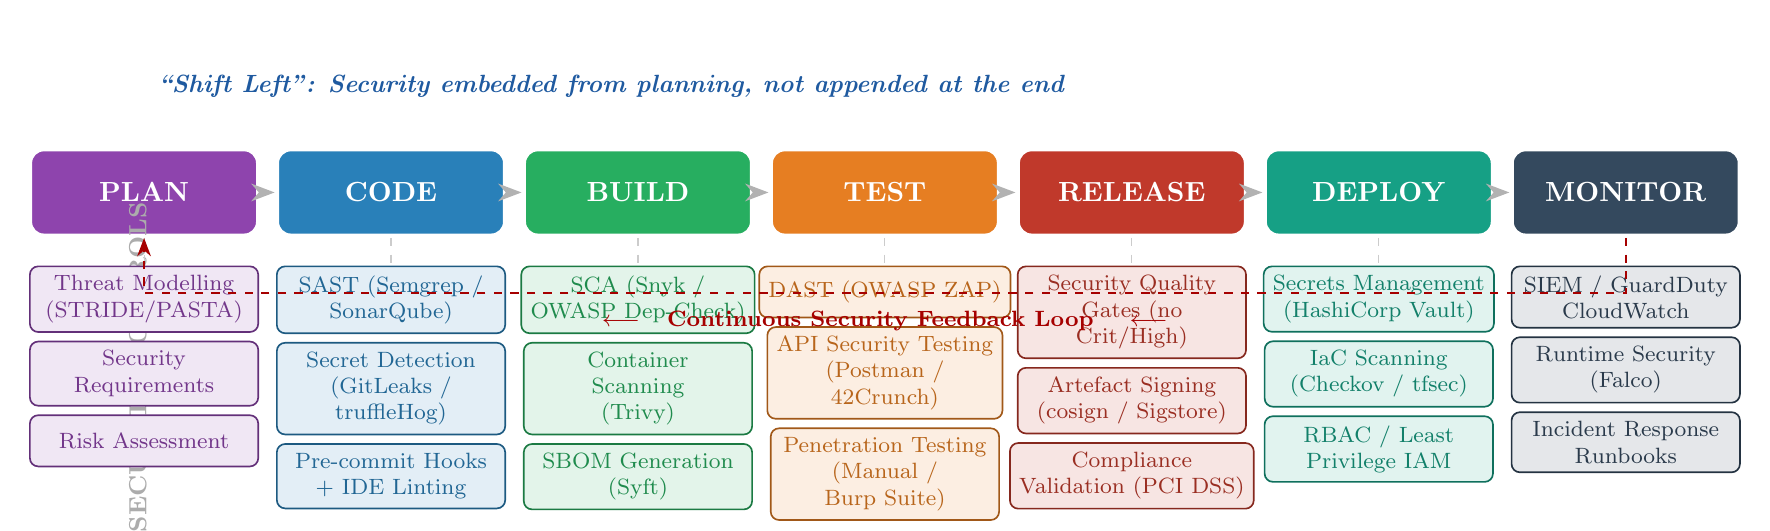
\begin{tikzpicture}[
    node distance=0.15cm and 0.15cm,
    phase/.style={
      rectangle, rounded corners=5pt,
      draw=white, ultra thick,
      fill=#1,
      minimum width=2.9cm, minimum height=1.1cm,
      text centered, text=white, font=\bfseries\normalsize
    },
    ctrl/.style={
      rectangle, rounded corners=3pt,
      draw=#1!70!black, line width=0.6pt,
      fill=#1!13,
      minimum width=2.9cm, minimum height=0.65cm,
      text centered, text=#1!80!black,
      font=\footnotesize, align=center
    },
    feedarr/.style={
      ->, >=Stealth, thick, draw=red!65!black, dashed
    },
    phasearr/.style={
      ->, >=Stealth, very thick, draw=gray!60
    }
  ]

  % ---- Phase header nodes ----
  \node[phase=cplan]    (PLAN)    {PLAN};
  \node[phase=ccode,    right=0.18cm of PLAN]    (CODE)    {CODE};
  \node[phase=cbuild,   right=0.18cm of CODE]   (BUILD)   {BUILD};
  \node[phase=ctest,    right=0.18cm of BUILD]   (TEST)    {TEST};
  \node[phase=crelease, right=0.18cm of TEST]    (RELEASE) {RELEASE};
  \node[phase=cdeploy,  right=0.18cm of RELEASE] (DEPLOY)  {DEPLOY};
  \node[phase=cmonitor, right=0.18cm of DEPLOY]  (MONITOR) {MONITOR};

  % ---- Arrows between phases ----
  \draw[phasearr] (PLAN.east)    -- (CODE.west);
  \draw[phasearr] (CODE.east)    -- (BUILD.west);
  \draw[phasearr] (BUILD.east)   -- (TEST.west);
  \draw[phasearr] (TEST.east)    -- (RELEASE.west);
  \draw[phasearr] (RELEASE.east) -- (DEPLOY.west);
  \draw[phasearr] (DEPLOY.east)  -- (MONITOR.west);

  % ---- Security section label ----
  \node[font=\small\bfseries\color{gray!65}, rotate=90,
        left=0.7cm of PLAN, yshift=-2.1cm] {SECURITY CONTROLS};

  % ---- PLAN controls ----
  \node[ctrl=cplan, below=0.35cm of PLAN]  (p1) {Threat Modelling\\(STRIDE/PASTA)};
  \node[ctrl=cplan, below=0.1cm of p1]     (p2) {Security\\Requirements};
  \node[ctrl=cplan, below=0.1cm of p2]     (p3) {Risk Assessment};

  % ---- CODE controls ----
  \node[ctrl=ccode, below=0.35cm of CODE]  (c1) {SAST (Semgrep /\\SonarQube)};
  \node[ctrl=ccode, below=0.1cm of c1]     (c2) {Secret Detection\\(GitLeaks /\\truffleHog)};
  \node[ctrl=ccode, below=0.1cm of c2]     (c3) {Pre-commit Hooks\\+ IDE Linting};

  % ---- BUILD controls ----
  \node[ctrl=cbuild, below=0.35cm of BUILD] (b1) {SCA (Snyk /\\OWASP Dep-Check)};
  \node[ctrl=cbuild, below=0.1cm of b1]     (b2) {Container\\Scanning\\(Trivy)};
  \node[ctrl=cbuild, below=0.1cm of b2]     (b3) {SBOM Generation\\(Syft)};

  % ---- TEST controls ----
  \node[ctrl=ctest, below=0.35cm of TEST]  (t1) {DAST (OWASP ZAP)};
  \node[ctrl=ctest, below=0.1cm of t1]     (t2) {API Security Testing\\(Postman /\\42Crunch)};
  \node[ctrl=ctest, below=0.1cm of t2]     (t3) {Penetration Testing\\(Manual /\\Burp Suite)};

  % ---- RELEASE controls ----
  \node[ctrl=crelease, below=0.35cm of RELEASE] (r1) {Security Quality\\Gates (no\\Crit/High)};
  \node[ctrl=crelease, below=0.1cm of r1]       (r2) {Artefact Signing\\(cosign / Sigstore)};
  \node[ctrl=crelease, below=0.1cm of r2]       (r3) {Compliance\\Validation (PCI DSS)};

  % ---- DEPLOY controls ----
  \node[ctrl=cdeploy, below=0.35cm of DEPLOY] (d1) {Secrets Management\\(HashiCorp Vault)};
  \node[ctrl=cdeploy, below=0.1cm of d1]      (d2) {IaC Scanning\\(Checkov / tfsec)};
  \node[ctrl=cdeploy, below=0.1cm of d2]      (d3) {RBAC / Least\\Privilege IAM};

  % ---- MONITOR controls ----
  \node[ctrl=cmonitor, below=0.35cm of MONITOR] (m1) {SIEM / GuardDuty\\CloudWatch};
  \node[ctrl=cmonitor, below=0.1cm of m1]       (m2) {Runtime Security\\(Falco)};
  \node[ctrl=cmonitor, below=0.1cm of m2]       (m3) {Incident Response\\Runbooks};

  % ---- Vertical connector lines (phase to first control) ----
  \foreach \ph/\ct in {PLAN/p1, CODE/c1, BUILD/b1, TEST/t1, RELEASE/r1, DEPLOY/d1, MONITOR/m1}{
    \draw[gray!40, dashed, thin] (\ph.south) -- (\ct.north);
  }

  % ---- Continuous Feedback Loop ----
  \draw[feedarr]
    (MONITOR.south)
    -- ++(0,-0.7) coordinate (br)
    -- (br -| PLAN.south) coordinate (bl)
    -- (PLAN.south);

  \node[font=\footnotesize\bfseries\color{red!65!black}]
    at ($(br)!0.5!(bl) + (0,-0.35)$)
    {$\longleftarrow$\quad Continuous Security Feedback Loop \quad$\longleftarrow$};

  % ---- "Shift Left" annotation ----
  \node[font=\small\bfseries\color{phaseblue}, above=0.5cm of CODE,
        xshift=2.8cm]
    {\textit{``Shift Left'': Security embedded from planning, not appended at the end}};

  \end{tikzpicture}
  }% end resizebox
  \caption{PayWave Digital --- Proposed Secure DevSecOps CI/CD Pipeline}
  \label{fig:pipeline}
\end{figure}
\end{landscape}

\subsection{Security Controls by Phase}

\subsubsection*{Phase 1 — Plan}

Every feature sprint begins with a structured threat modelling session using the STRIDE
framework to enumerate threats applicable to PayWave's payment APIs and microservice
interactions. Security requirements derived from threat models, PCI DSS obligations
\citep{pciDSS2022}, and the OWASP ASVS \citep{owaspasvs} are documented as acceptance
criteria in Jira tickets, ensuring that security is a first-class functional requirement rather than an
afterthought.

\subsubsection*{Phase 2 — Code}

SAST is integrated into the GitHub Actions workflow and developer IDEs via SonarLint. Every
commit triggers Semgrep rules customised for Python, Node.js, and Java microservices.
Critically for PayWave, pre-commit hooks enforced via \texttt{.pre-commit-config.yaml} run
GitLeaks and truffleHog to detect hard-coded secrets, API keys, and private credentials
before they enter version control --- directly addressing the incident identified during
investor due diligence. Peer code review is mandated for all changes to security-sensitive
modules (authentication, payment processing, API gateways).

\subsubsection*{Phase 3 — Build}

Software Composition Analysis using Snyk and OWASP Dependency-Check scans all third-party
libraries and transitive dependencies against the NVD and GitHub Advisory Database on every
build. Container images are scanned with Trivy \citep{trivy2023} for OS-level and
library-level vulnerabilities before being pushed to the container registry. An SBOM is
generated using Syft for every release artefact, enabling PayWave to respond rapidly to
future supply chain vulnerability disclosures. Builds with critical or high-severity
unresolved findings fail automatically.

\subsubsection*{Phase 4 — Test}

DAST is performed against the staging environment using OWASP ZAP in automated scan mode
within the GitHub Actions pipeline, targeting all publicly exposed REST API endpoints and
the customer-facing web application. API security testing using Postman/Newman or 42Crunch
validates that JWT authentication, authorisation boundaries, and rate-limiting controls
function correctly. Quarterly manual penetration testing by an external firm provides
deeper coverage of business-logic vulnerabilities that automated tools cannot reliably
detect.

\subsubsection*{Phase 5 — Release}

Automated security quality gates prevent promotion to production unless all critical and
high-severity findings from SAST, SCA, and DAST phases are resolved or formally accepted.
Release artefacts (container images, Helm charts) are cryptographically signed using
Sigstore's \texttt{cosign}, ensuring supply chain integrity from build to deployment.

\subsubsection*{Phase 6 — Deploy}

HashiCorp Vault \citep{hashicorpvault} provides centralised secrets management, injecting
database credentials, payment gateway API keys, and internal service tokens into running
containers at runtime via the Vault Agent Sidecar --- eliminating hard-coded credentials
entirely. Infrastructure-as-code templates (Terraform/CloudFormation) are scanned with
Checkov and tfsec before deployment to detect misconfigurations (open security groups,
public S3 buckets, missing encryption). AWS IAM roles follow least-privilege principles,
enforced through automated policy validation.

\subsubsection*{Phase 7 — Monitor}

AWS CloudWatch and GuardDuty provide cloud-native threat detection, with Falco installed as
a Kubernetes DaemonSet for container runtime security monitoring. Anomalous API access
patterns, authentication anomalies, and unusual data transfer volumes trigger automated
alerts routed to the Security Operations team via PagerDuty. Findings feed back into the
threat model and backlog through a weekly security review meeting, closing the continuous
improvement loop illustrated in Figure~\ref{fig:pipeline}.

\newpage

% ============================================================
% QUESTION 3 — STRIDE Threat Modelling (15 marks)
% ============================================================
\section{Threat Modelling: STRIDE Analysis for Healthcare API Platform}

\begin{secbox}{Scenario}
An organisation is deploying a cloud-native healthcare API platform that stores and exposes
patient medical records. The STRIDE framework is applied to identify one realistic threat
per category, its CIA impact, and a recommended mitigation.
\end{secbox}

\subsection{STRIDE Threat Analysis}

\renewcommand{\arraystretch}{1.55}
\begin{longtable}{>{\bfseries\color{phaseblue}}p{2.6cm}
                   p{4.2cm}
                   p{3.4cm}
                   p{4.1cm}}
\toprule
\normalfont\textbf{\color{phaseblue}STRIDE Category} &
\textbf{Threat Scenario} &
\textbf{CIA Impact} &
\textbf{Mitigation Strategy} \\
\midrule
\endfirsthead
\toprule
\normalfont\textbf{\color{phaseblue}STRIDE Category} &
\textbf{Threat Scenario} &
\textbf{CIA Impact} &
\textbf{Mitigation Strategy} \\
\midrule
\endhead
\bottomrule
\endfoot

\rowcolor{cplan!8}
\shortstack[l]{Spoofing\\Identity} &
An attacker obtains a stolen OAuth 2.0 access token via phishing and replays it to
authenticate as a legitimate clinician, accessing the patient records API without
authorisation. &
\textbf{Confidentiality:} Unauthorised access to protected health information (PHI) violates POPIA
\citep{popia2013} and HIPAA, risking regulatory sanction and patient harm. &
Implement short-lived JWT tokens (15-min expiry) with rotating refresh tokens; enforce
multi-factor authentication (MFA) for all API access; deploy token revocation lists and
anomalous usage detection. \\

\midrule
\rowcolor{ccode!7}
\shortstack[l]{Tampering\\with Data} &
A man-in-the-middle (MITM) attacker intercepts unencrypted API traffic between a hospital
system and the cloud API, modifying a patient's medication dosage field before it reaches
the records database. &
\textbf{Integrity:} Falsified medical records could lead to incorrect clinical decisions,
medication errors, and patient harm. &
Enforce TLS 1.3 with HSTS for all API communications; apply HTTP Strict Transport Security
(HSTS); implement digital signatures (HMAC-SHA256) on critical record payloads to detect
in-transit tampering. \\

\midrule
\rowcolor{cbuild!7}
\shortstack[l]{Repudiation} &
A healthcare professional accesses and modifies a patient's diagnosis records, then later
claims the action was unauthorised or performed by another user, exploiting an absence of
reliable audit trails. &
\textbf{Integrity:} Without non-repudiation, accountability is impossible; investigations
into data misuse or clinical negligence cannot be substantiated. &
Implement immutable, cryptographically signed audit logs stored in a tamper-evident
ledger (e.g., AWS CloudTrail with log file validation); include actor identity,
timestamp, and record hash in every write event. \\

\midrule
\rowcolor{ctest!7}
\shortstack[l]{Information\\Disclosure} &
An authenticated low-privilege patient portal user exploits an Insecure Direct Object
Reference (IDOR) vulnerability by incrementing record IDs in API requests, successfully
retrieving other patients' complete medical histories. &
\textbf{Confidentiality:} Mass exposure of third-party PHI constitutes a notifiable data
breach under POPIA Section~22 \citep{popia2013}, incurring regulatory penalties and reputational damage. &
Enforce object-level authorisation on every API endpoint; implement Attribute-Based Access
Control (ABAC) ensuring records are accessible only to their owning patient or authorised
clinicians; conduct IDOR-specific security testing. \\

\midrule
\rowcolor{crelease!7}
\shortstack[l]{Denial of\\Service} &
An adversary launches a volumetric DDoS attack, flooding the patient records API with
millions of requests per second, rendering the platform unavailable to clinical staff
during an emergency response scenario. &
\textbf{Availability:} Inability of clinical staff to access patient records in time-critical
situations directly endangers patient lives, constituting a severe patient safety incident. &
Deploy AWS WAF with rate-based rules and AWS Shield Advanced for DDoS mitigation; implement
API gateway-level rate limiting and circuit breakers; configure auto-scaling with surge
protection; utilise a CDN to absorb volumetric traffic. \\

\midrule
\rowcolor{cdeploy!7}
\shortstack[l]{Elevation of\\Privilege} &
An attacker exploits a broken function-level authorisation vulnerability, sending an API
request with a manipulated \texttt{role} field to escalate from a read-only patient user
to an administrator, gaining full CRUD access to all patient records. &
\textbf{Confidentiality \& Integrity:} The attacker can read, modify, and delete arbitrary
patient records, causing data integrity violations and mass PHI exposure simultaneously. &
Enforce Role-Based Access Control (RBAC) validated server-side on every request,
independent of client-supplied parameters; apply the principle of least privilege; use
established authorisation frameworks (OPA/Casbin); include privilege escalation scenarios
in regular penetration testing. \\

\bottomrule
\end{longtable}
\renewcommand{\arraystretch}{1}

\subsection{Why Threat Modelling Must Precede Penetration Testing}

Threat modelling and penetration testing serve complementary but fundamentally different
purposes in a security programme. Several reasons justify performing threat modelling
\emph{before} penetration testing:

\begin{itemize}
  \item \textbf{Proactive versus reactive posture.} Threat modelling is a proactive,
    design-time activity that systematically enumerates potential attack vectors before
    any code is written. Penetration testing is reactive and binary --- it probes a
    completed system for exploitable flaws. By the time a penetration tester identifies
    an architectural flaw (such as missing authentication on an internal API endpoint),
    fixing it may require significant rework of live systems \citep{howard2006}.

  \item \textbf{Cost of remediation.} Architectural security flaws identified during
    design are orders of magnitude cheaper to remediate than those discovered post-
    deployment. A design-level threat model can redirect architectural decisions before
    a single line of code is committed \citep{ibm2012}.

  \item \textbf{Completeness and coverage.} Penetration testing is inherently time-
    bounded and samples the attack surface rather than comprehensively covering it.
    Threat modelling systematically enumerates all trust boundaries, data flows, and
    assets, producing a structured register of threats against which countermeasures can
    be verified. Penetration testing then validates whether the countermeasures are
    correctly implemented.

  \item \textbf{Design influence.} Many critical security controls (separation of
    concerns, privilege separation, data classification, encryption boundaries) can only
    be meaningfully influenced at the architecture and design stage. A penetration test
    on a deployed system cannot change its fundamental trust model.

  \item \textbf{Informed scoping.} Threat models produce structured threat registers
    that allow penetration testers to focus effort on the highest-risk attack paths,
    improving both the efficiency and depth of testing engagements.
\end{itemize}

In summary, threat modelling defines \emph{what} should be secure and \emph{why}, while
penetration testing validates \emph{whether} the implemented controls achieve that goal.
Neither substitutes for the other; but threat modelling must come first.

\newpage

% ============================================================
% QUESTION 4 — OWASP ZAP Practical Lab (25 marks)
% ============================================================
\section{Practical DevSecOps Lab: OWASP ZAP Vulnerability Assessment}

% ----
\subsection{Introduction}

This report documents a Dynamic Application Security Testing (DAST) exercise performed
using OWASP ZAP \citep{owaspzap} against the OWASP Juice Shop
\citep{owaspjuiceshop} --- a deliberately vulnerable web application designed for security
training. The objective was to demonstrate automated vulnerability discovery within a
DevSecOps context, identify real-world application security weaknesses, and evaluate the
effectiveness of DAST as a pipeline control. The scan was performed on \textbf{11 May
2026} against a locally hosted Juice Shop instance at \texttt{http://localhost:3000}. The
assessment identified one \textbf{High}-risk vulnerability (SQL Injection) and multiple
\textbf{Medium}-risk findings relating to Content Security Policy (CSP),
cross-domain configuration (CORS), and session identifiers exposed in URLs.

% ----
\subsection{Environment Setup}

\subsubsection*{Target Application: OWASP Juice Shop}

OWASP Juice Shop was deployed locally using Docker:

\begin{lstlisting}[language=bash, caption={Deploy OWASP Juice Shop via Docker}]
docker pull bkimminich/juice-shop
docker run -d -p 3000:3000 bkimminich/juice-shop
\end{lstlisting}

The application was accessible at \texttt{http://localhost:3000}. Juice Shop is a
Node.js/Express single-page application intentionally containing OWASP Top 10
vulnerabilities, making it an ideal DAST training target.

\begin{figure}[H]
  \centering
  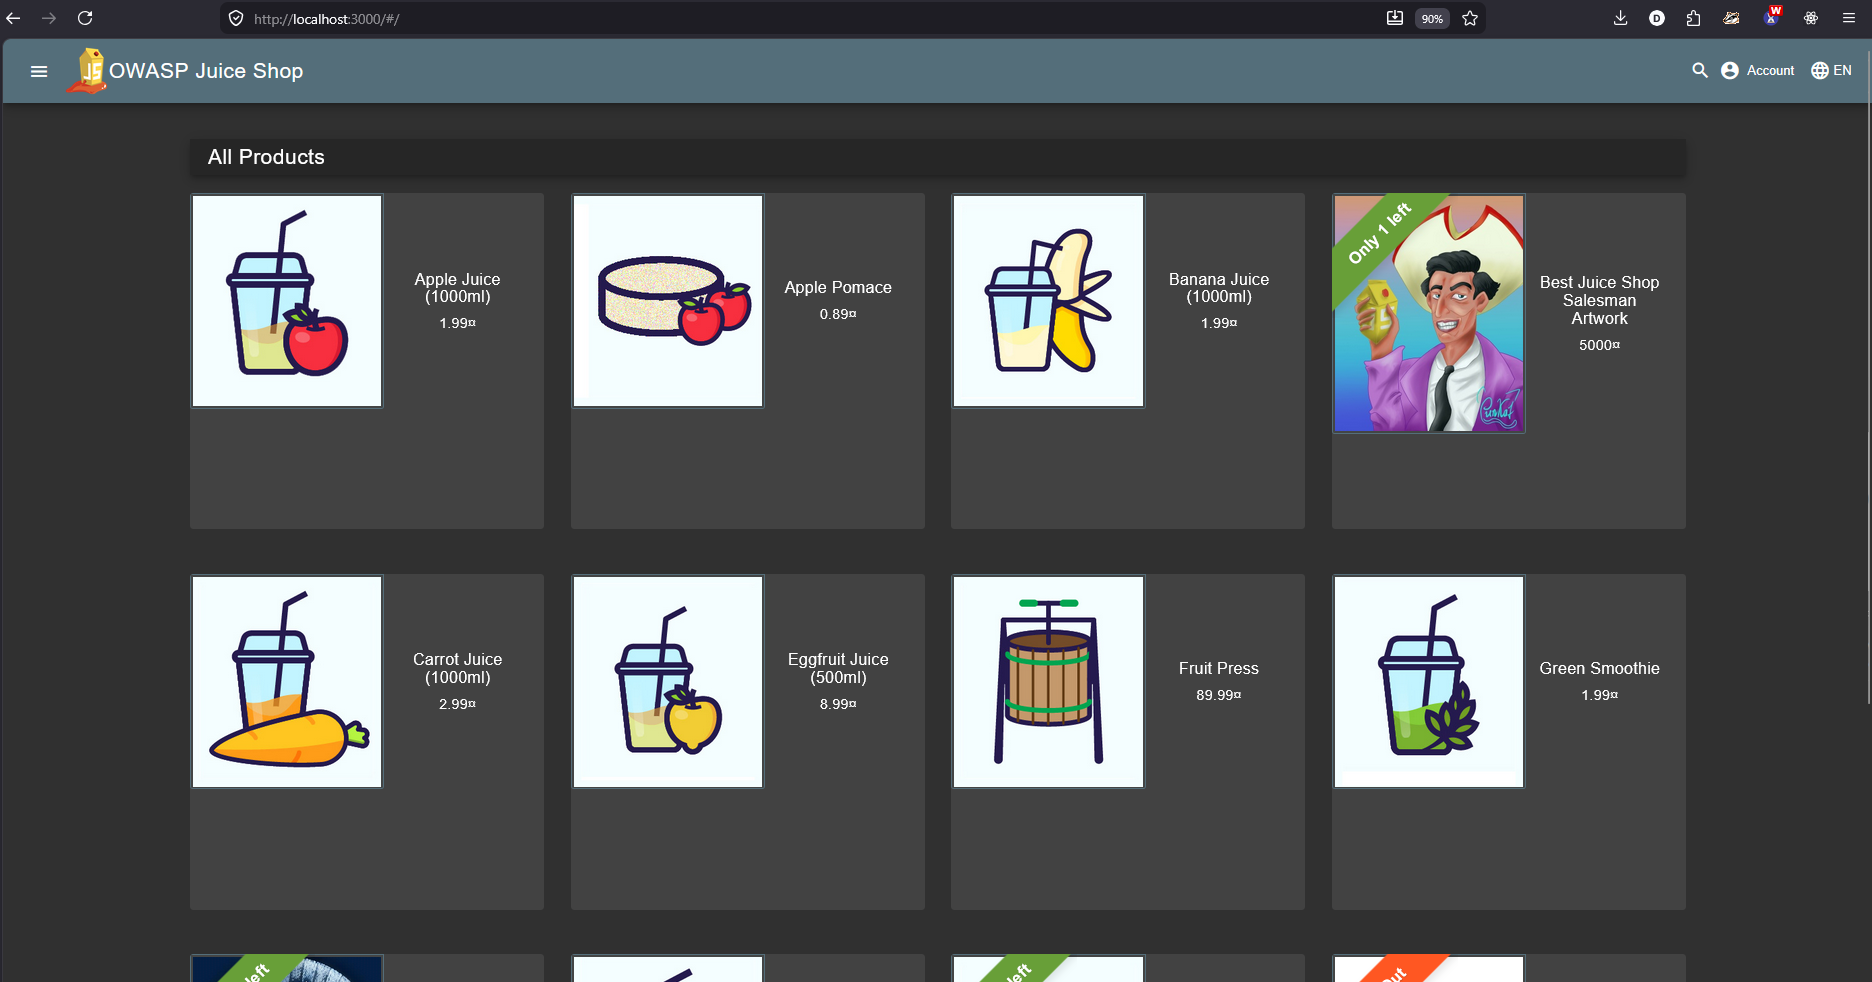
\includegraphics[width=\textwidth]{image.png}
  \caption{OWASP Juice Shop running locally at \texttt{http://localhost:3000}.}
  \label{fig:juiceshop}
\end{figure}

\subsubsection*{OWASP ZAP Installation}

OWASP ZAP (version 2.14+) was downloaded from \texttt{https://www.zaproxy.org/download/}
and installed on the host machine. The Community Edition provides all features required for
this assessment.

\subsubsection*{Proxy Configuration}

ZAP was configured as an intercepting proxy:
\begin{enumerate}
  \item ZAP proxy listener set to \texttt{localhost:8080} (Tools $\to$ Options $\to$
    Network $\to$ Local Servers/Proxies).
  \item Firefox configured to use a manual proxy (\texttt{localhost:8080}) for HTTP and
    HTTPS traffic so that requests pass through ZAP for inspection and scanning.
\end{enumerate}

\begin{figure}[H]
  \centering
  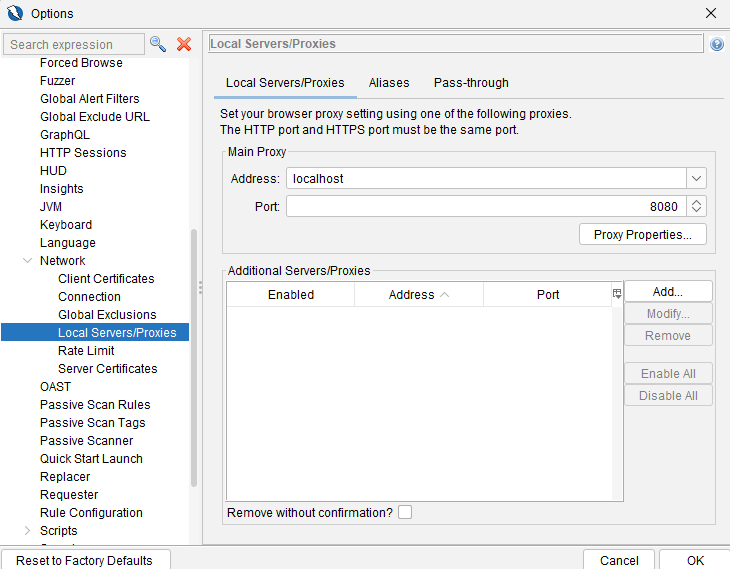
\includegraphics[width=0.85\textwidth]{image copy 11.png}
  \caption{ZAP local proxy listener configured on \texttt{localhost:8080}.}
  \label{fig:zap-proxy}
\end{figure}

\begin{figure}[H]
  \centering
  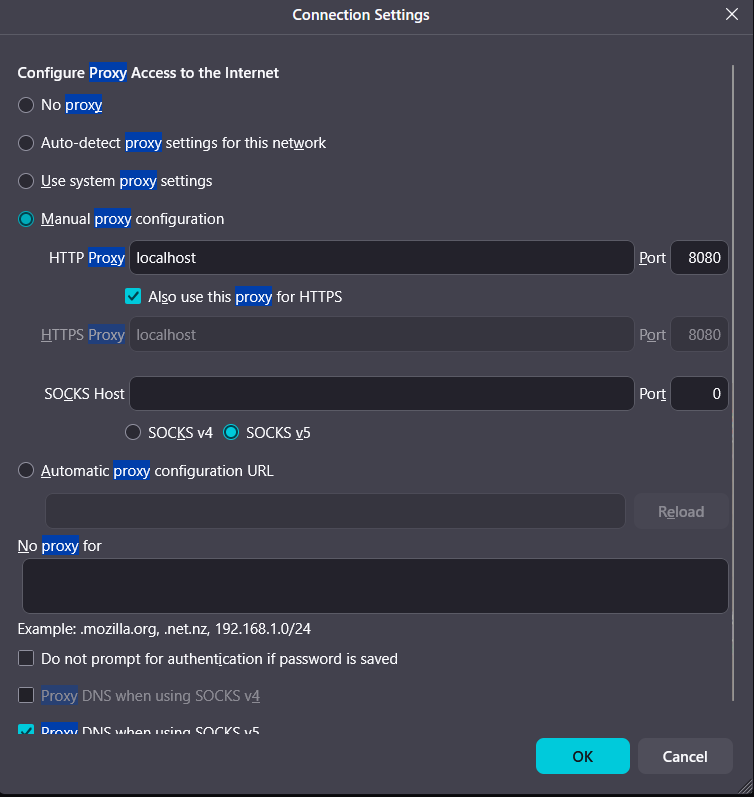
\includegraphics[width=0.85\textwidth]{image copy 12.png}
  \caption{Firefox manual proxy settings pointing to \texttt{localhost:8080}.}
  \label{fig:firefox-proxy}
\end{figure}

% ----
\subsection{Scan Configuration}

\subsubsection*{Traditional Spider (Crawling)}

The Traditional Spider was launched against \texttt{http://localhost:3000}:
\begin{itemize}
  \item Navigate to: \textit{Tools $\to$ Spider $\to$ New Scan}
  \item Starting URL: \texttt{http://localhost:3000}
  \item Results: \textbf{385 URLs found} and \textbf{274 nodes added} (including REST API
    endpoints, static assets, and application routes).
\end{itemize}

\begin{figure}[H]
  \centering
  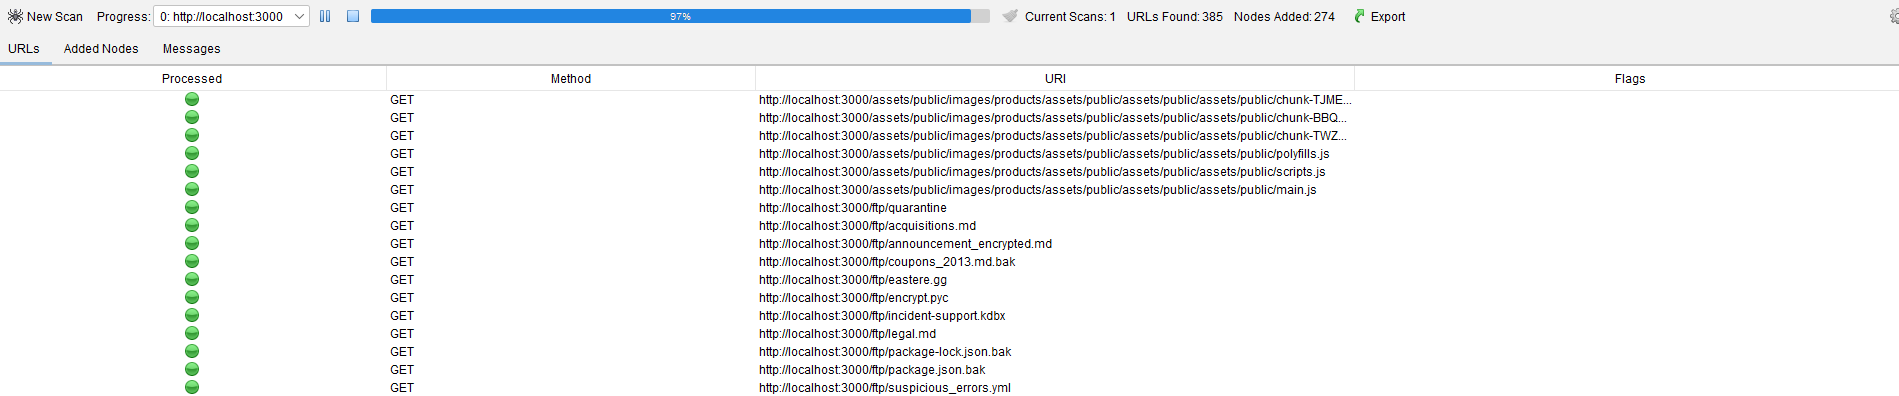
\includegraphics[width=\textwidth]{image copy.png}
  \caption{Traditional spider results showing discovered URLs and endpoints.}
  \label{fig:zap-spider}
\end{figure}

\textbf{Note on AJAX Spider.}
Because Juice Shop is an Angular-based Single Page Application (SPA), OWASP ZAP's
\textit{AJAX Spider} is available as a complement to the Traditional Spider. The AJAX
Spider executes JavaScript, follows client-side routes, and interacts with dynamic content,
providing deeper coverage of modern SPA architectures. Combined use of both spiders is
recommended for production-grade assessments against JavaScript-heavy applications.

\subsubsection*{Active Scan}

Following the spider, an Active Scan was launched to probe discovered endpoints for
vulnerabilities:
\begin{itemize}
  \item Navigate to: \textit{Tools $\to$ Active Scan $\to$ New Scan}
  \item Target: \texttt{http://localhost:3000}
  \item Scan Policy: Default Active Scan Policy
  \item The active scan generated large volumes of requests and flagged new alerts as it
    tested the discovered attack surface.
\end{itemize}

\begin{figure}[H]
  \centering
  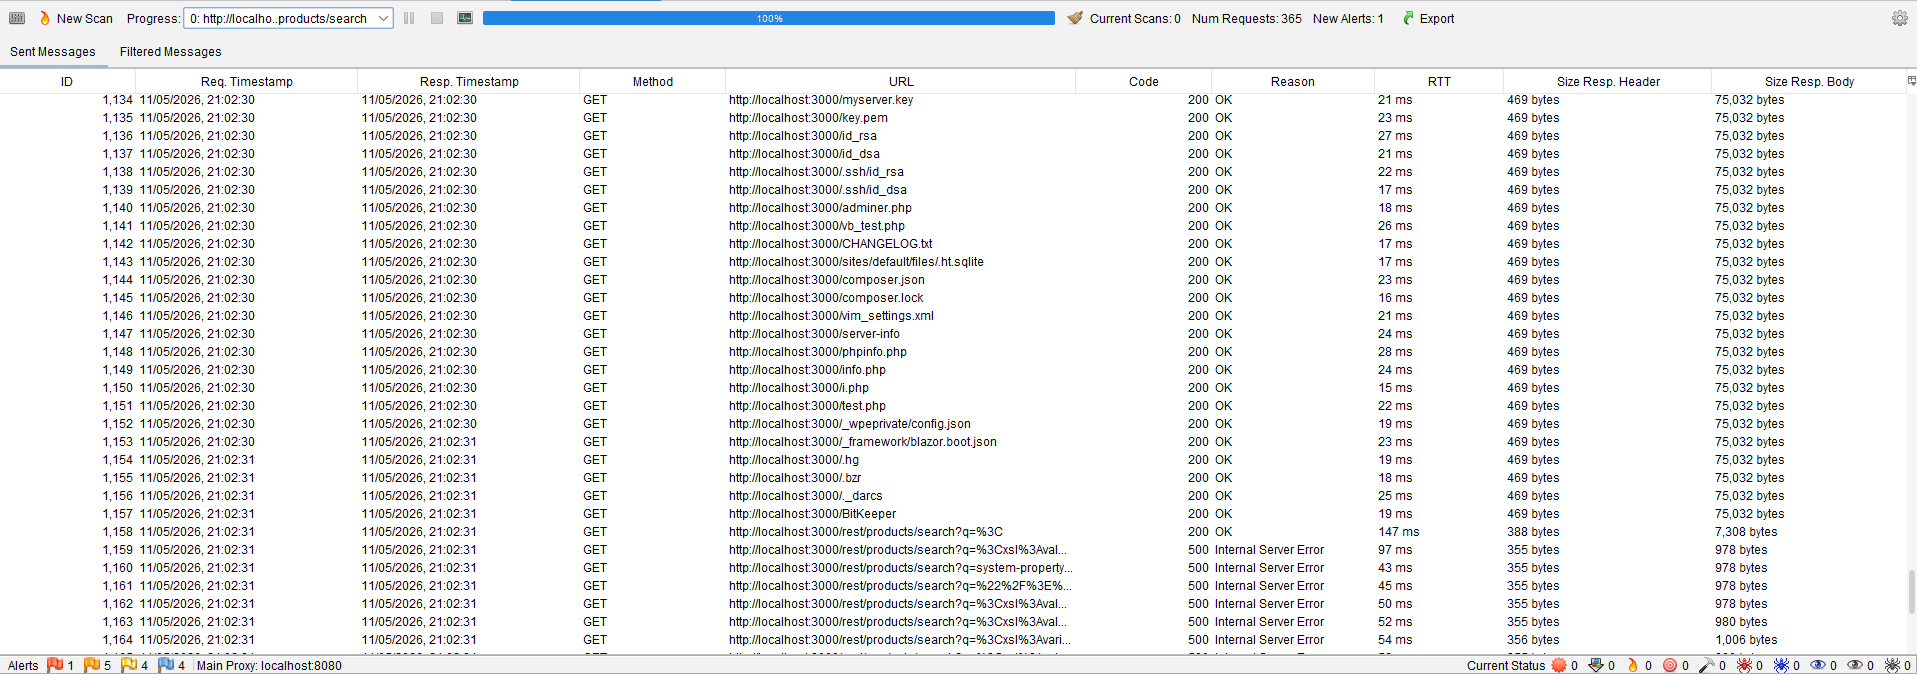
\includegraphics[width=\textwidth]{image copy 10.png}
  \caption{Active scanning traffic recorded in ZAP (requests and server responses).}
  \label{fig:zap-active-scan}
\end{figure}

% ----
\subsection{Findings}

The automated scan produced the following security findings. The complete Alerts list in
ZAP is shown in Figure~\ref{fig:alerts}.

\begin{figure}[H]
  \centering
  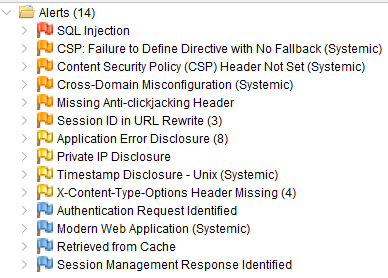
\includegraphics[width=0.7\textwidth]{image copy 2.png}
  \caption{ZAP Alerts list for the Juice Shop scan (grouped by risk level).}
  \label{fig:alerts}
\end{figure}

\subsubsection*{Finding 1 --- SQL Injection [HIGH RISK]}

\begin{warnbox}{\textcolor{highred}{\textbf{HIGH RISK:}} SQL Injection}
\begin{tabular}{@{}ll@{}}
\textbf{Risk Level:}   & \textcolor{highred}{\textbf{High}} \\
\textbf{CWE:}          & CWE-89 --- Improper Neutralisation of SQL Commands \\
\textbf{OWASP 2021:}   & A03:2021 --- Injection \\
\textbf{Affected URL:} & \texttt{GET http://localhost:3000/rest/products/search} \\
\textbf{Parameter:}    & \texttt{q} \\
\textbf{Evidence:}     & Crafted input triggered \texttt{HTTP/1.1 500 Internal Server Error}
                         during scanning \\
\end{tabular}
\end{warnbox}

\textbf{Vulnerability Type.}
SQL Injection (SQLi) occurs when untrusted user-supplied input is incorporated directly
into a database query without adequate sanitisation or parameterisation. An attacker can
manipulate the query logic to bypass authentication, extract arbitrary data, modify records,
or in some configurations, execute operating system commands \citep{owasp2021top10}.

\textbf{Risk Impact.}
In this assessment, ZAP flagged a potential SQL injection in the Juice Shop product search
endpoint \texttt{/rest/products/search} (parameter \texttt{q}). The alert evidence shows
server errors when crafted payloads were submitted, which is commonly associated with
error-based SQLi detection and warrants manual verification. In a production payment
platform such as PayWave, a confirmed SQL injection would enable:
\begin{itemize}
  \item Unauthorised extraction of sensitive data (PII, accounts, transaction history).
  \item Integrity compromise by modifying records (e.g., balances, beneficiary details).
  \item Potential disruption of service availability through destructive queries.
\end{itemize}
The CVSS v3.1 base score for a remotely exploitable SQL injection is often
\textbf{High--Critical} (worst-case \textbf{9.8}).

\begin{figure}[H]
  \centering
  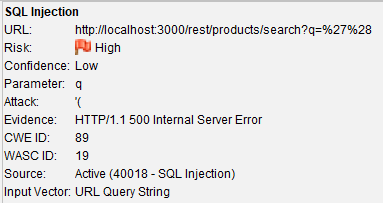
\includegraphics[width=0.7\textwidth]{image copy 3.png}
  \caption{SQL Injection alert details raised by ZAP for \texttt{/rest/products/search}.}
  \label{fig:sqli}
\end{figure}

\textbf{Mitigation Strategy.}
\begin{itemize}
  \item \textbf{Parameterised queries / prepared statements}: Replace all dynamic SQL
    string concatenation with parameterised queries using the ORM's bound-parameter API
    (e.g., Sequelize query builders with bound parameters rather than raw SQL strings).
  \item \textbf{Input validation}: Validate and sanitise all user inputs at the
    application boundary; reject inputs containing SQL metacharacters (\texttt{' -- ;}).
  \item \textbf{Principle of least privilege}: The database user account used by the
    application should have minimal permissions (SELECT/INSERT/UPDATE only; no DROP or
    administrative functions).
  \item \textbf{Web Application Firewall (WAF)}: Deploy AWS WAF with SQL injection
    detection rules as a defence-in-depth layer.
  \item \textbf{SAST enforcement}: Enforce SAST rules (Semgrep \texttt{sql-injection}
    ruleset) in the CI pipeline to prevent injection-prone code patterns from merging.
\end{itemize}

% ----

\subsubsection*{Finding 2 --- Content Security Policy (CSP) Header Not Set [MEDIUM RISK]}

\begin{secbox}{\textcolor{medorange}{\textbf{MEDIUM RISK:}} Content Security Policy (CSP) Header Not Set}
\begin{tabular}{@{}ll@{}}
\textbf{Risk Level:}   & \textcolor{medorange}{\textbf{Medium}} \\
\textbf{CWE:}          & CWE-693 --- Protection Mechanism Failure \\
\textbf{OWASP 2021:}   & A05:2021 --- Security Misconfiguration \\
\textbf{Affected URL:} & \texttt{GET http://localhost:3000/socket.io/} \\
\textbf{Evidence:}     & \texttt{Content-Security-Policy} response header absent \\
\end{tabular}
\end{secbox}

\textbf{Vulnerability Type.}
The \texttt{Content-Security-Policy} (CSP) HTTP response header instructs browsers which
sources of scripts, styles, frames, and other resources are trusted for a given page. When
absent, browsers operate in their default permissive mode, permitting execution of
injected scripts from any origin \citep{owasp2021top10}.

\textbf{Risk Impact.}
Without a CSP header:
\begin{itemize}
  \item Reflected and Stored XSS attacks can execute arbitrary JavaScript in victims'
    browsers, enabling session token theft, credential harvesting, and DOM manipulation.
  \item Malicious third-party scripts injected via supply chain compromise (e.g., a
    compromised npm CDN package) will execute unchallenged.
  \item Clickjacking attacks via \texttt{<iframe>} embedding remain possible.
  \item In a payment context such as PayWave, XSS combined with an absent CSP could
    enable attackers to silently redirect payment flows to attacker-controlled endpoints.
\end{itemize}

\begin{figure}[H]
  \centering
  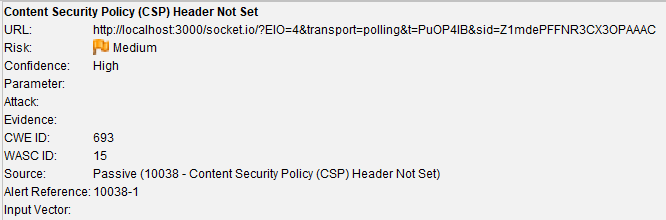
\includegraphics[width=0.7\textwidth]{image copy 5.png}
  \caption{ZAP alert showing \texttt{Content-Security-Policy} header not set (Medium).}
  \label{fig:csp-header-not-set}
\end{figure}

\textbf{Mitigation Strategy.}
\begin{itemize}
  \item Add a \texttt{Content-Security-Policy} header to all HTTP responses, beginning
    with a restrictive policy such as:
\begin{lstlisting}
Content-Security-Policy: default-src 'self';
  script-src 'self' https://trusted-cdn.com;
  object-src 'none'; frame-ancestors 'none';
\end{lstlisting}
  \item Use \texttt{Content-Security-Policy-Report-Only} initially to audit policy
    effectiveness before enforcement.
  \item Combine with \texttt{X-Frame-Options: DENY} and
    \texttt{X-Content-Type-Options: nosniff} for defence-in-depth.
  \item Enforce CSP header presence in automated pipeline testing (ZAP passive scan rules).
\end{itemize}

% ----

\subsubsection*{Finding 3 --- CSP: Failure to Define Directive with No Fallback [MEDIUM RISK]}

\begin{secbox}{\textcolor{medorange}{\textbf{MEDIUM RISK:}} CSP Directive Missing Fallback}
\begin{tabular}{@{}ll@{}}
\textbf{Risk Level:}   & \textcolor{medorange}{\textbf{Medium}} \\
\textbf{CWE:}          & CWE-693 --- Protection Mechanism Failure \\
\textbf{OWASP 2021:}   & A05:2021 --- Security Misconfiguration \\
\textbf{Affected URL:} & \texttt{http://localhost:3000/assets/public/images/products} \\
\textbf{Evidence:}     & CSP directive without fallback not defined (systemic) \\
\end{tabular}
\end{secbox}

\textbf{Vulnerability Type.}
Some CSP directives (for example \texttt{frame-ancestors}) do not fall back to
\texttt{default-src}. If such directives are omitted, the browser may apply permissive
defaults, weakening protections against framing and related attacks.

\textbf{Risk Impact.}
\begin{itemize}
  \item Increased exposure to clickjacking (framing) if \texttt{frame-ancestors} is not
    explicitly restricted.
  \item Reduced defence-in-depth against script injection where CSP should constrain trusted
    sources.
  \item In payment contexts, UI redressing and script execution can be leveraged to trick
    users into unauthorised actions.
\end{itemize}

\begin{figure}[H]
  \centering
  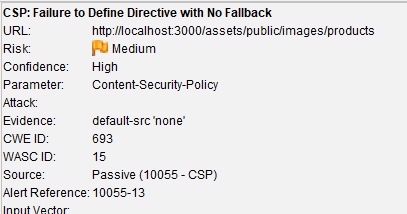
\includegraphics[width=0.7\textwidth]{image copy 4.png}
  \caption{ZAP alert: CSP directive failure to define directive with no fallback (Medium).}
  \label{fig:csp-nofallback}
\end{figure}

\textbf{Mitigation Strategy.}
\begin{itemize}
  \item Apply a complete CSP policy across the application, ensuring directives without
    fallback are explicitly set (e.g., \texttt{frame-ancestors 'none'}).
  \item Start with \texttt{Content-Security-Policy-Report-Only} to validate compatibility,
    then enforce once stable.
  \item Validate CSP consistency with automated DAST (ZAP passive scan) as a CI gate.
\end{itemize}

% ----

\subsubsection*{Finding 4 --- Cross-Domain Misconfiguration (Permissive CORS) [MEDIUM RISK]}

\begin{secbox}{\textcolor{medorange}{\textbf{MEDIUM RISK:}} Cross-Domain Misconfiguration (CORS)}
\begin{tabular}{@{}ll@{}}
\textbf{Risk Level:}   & \textcolor{medorange}{\textbf{Medium}} \\
\textbf{CWE:}          & CWE-264 --- Permissions, Privileges, and Access Controls \\
\textbf{OWASP 2021:}   & A01:2021 --- Broken Access Control \\
\textbf{Affected URL:} & \texttt{http://localhost:3000/chunk-*.js} \\
\textbf{Evidence:}     & \texttt{Access-Control-Allow-Origin: *} \\
\end{tabular}
\end{secbox}

\textbf{Vulnerability Type.}
Cross-Origin Resource Sharing (CORS) controls which origins (domains) are allowed to read
responses in a browser context. A wildcard policy can be unsafe if applied to endpoints
serving sensitive data or allowing authenticated requests.

\textbf{Risk Impact.}
\begin{itemize}
  \item When enabled on sensitive API endpoints, permissive CORS can enable cross-site data
    access from attacker-controlled web origins.
  \item In a payments platform, this may contribute to exposure of customer or transaction
    data to malicious websites.
\end{itemize}

\begin{figure}[H]
  \centering
  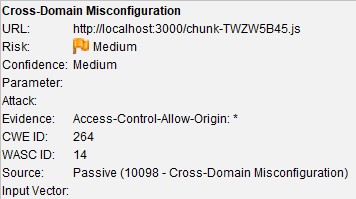
\includegraphics[width=0.7\textwidth]{image copy 6.png}
  \caption{ZAP alert highlighting \texttt{Access-Control-Allow-Origin: *} (Medium).}
  \label{fig:cors}
\end{figure}

\textbf{Mitigation Strategy.}
\begin{itemize}
  \item Restrict allowed origins to an explicit allow-list and only enable CORS where it is
    required.
  \item Avoid enabling wildcard CORS on authenticated endpoints; rely on the Same Origin
    Policy by default.
  \item Re-test with ZAP after configuration changes to confirm remediation.
\end{itemize}

% ----

\subsubsection*{Additional Medium Finding --- Session ID in URL Rewrite}

ZAP also flagged \textbf{Session ID in URL Rewrite} (Medium), indicating that a session
identifier was observed in the URL as a \texttt{sid} parameter. Session identifiers in
URLs can leak via browser history, logs, and the \texttt{Referer} header, increasing the
risk of session hijacking.

\begin{figure}[H]
  \centering
  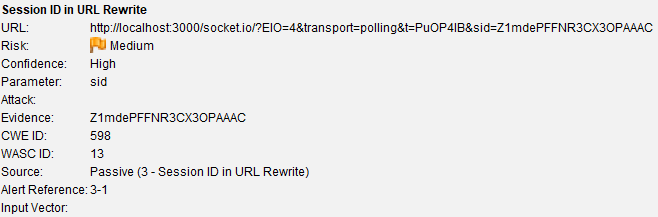
\includegraphics[width=0.7\textwidth]{image copy 7.png}
  \caption{Session identifier observed in the URL (\texttt{sid} parameter).}
  \label{fig:sid-url}
\end{figure}

\subsubsection*{Other Findings (Low/Informational)}

ZAP also reported lower-priority findings that were not part of the required High/Medium
minimum counts:
\begin{itemize}
  \item \textbf{Timestamp Disclosure (Unix) [Low]:} a Unix timestamp value was disclosed in
    responses, which may help attackers infer build/deploy timing or internal behaviour.
  \item \textbf{Modern Web Application [Informational]:} identifies modern front-end
    behaviour (e.g., SPA scripting) and is primarily informational.
\end{itemize}

\begin{figure}[H]
  \centering
  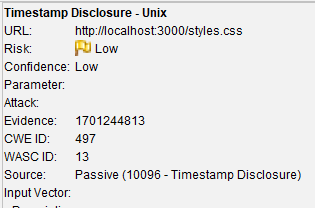
\includegraphics[width=0.7\textwidth]{image copy 8.png}
  \caption{Low-risk finding: Timestamp Disclosure (Unix).}
  \label{fig:timestamp}
\end{figure}

\begin{figure}[H]
  \centering
  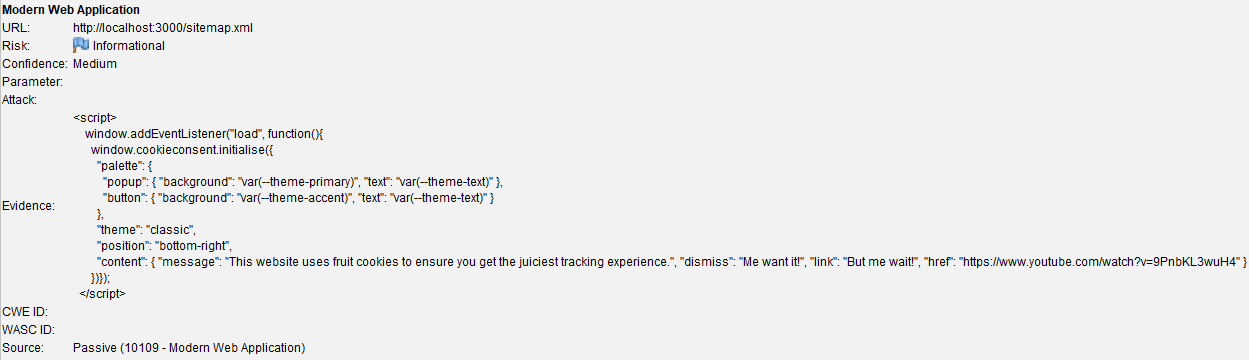
\includegraphics[width=\textwidth]{image copy 9.png}
  \caption{Informational finding: Modern Web Application indicator.}
  \label{fig:modern-web-app}
\end{figure}

% ----
\subsection{Risk Analysis Summary}

\begin{center}
\renewcommand{\arraystretch}{1.4}
\begin{tabularx}{\textwidth}{lXllX}
\toprule
\textbf{\#} & \textbf{Vulnerability} & \textbf{Risk} & \textbf{CVSS} & \textbf{Primary Impact} \\
\midrule
1 & SQL Injection & \textcolor{highred}{\textbf{High}} & 9.8 &
  Database compromise; unauthorised data access \\
2 & CSP Header Not Set & \textcolor{medorange}{\textbf{Medium}} & 6.1 &
  Increased XSS/clickjacking exposure due to missing browser policy \\
3 & CSP Directive Missing Fallback & \textcolor{medorange}{\textbf{Medium}} & 5.3 &
  Weak framing controls and reduced defence-in-depth \\
4 & Cross-Domain Misconfiguration (CORS) & \textcolor{medorange}{\textbf{Medium}} & 6.5 &
  Cross-origin data exposure risk if applied to sensitive endpoints \\
5 & Session ID in URL Rewrite & \textcolor{medorange}{\textbf{Medium}} & 6.5 &
  Session leakage via URLs (history/logs/\texttt{Referer}) \\
\bottomrule
\end{tabularx}
\renewcommand{\arraystretch}{1}
\end{center}

% ----
\subsection{Mitigation Recommendations Summary}

\begin{enumerate}
  \item \textbf{Immediate (Critical):} Replace all raw SQL string interpolation with
    parameterised ORM queries. Apply input validation on all user-facing endpoints.
    Deploy WAF rules to detect and block SQL injection patterns. Re-test with ZAP after
    remediation.

  \item \textbf{Short-term (High Priority):} Configure a complete
    \texttt{Content-Security-Policy} (including directives without fallback such as
    \texttt{frame-ancestors}) and ensure it is consistently applied across all application
    paths (including \texttt{/socket.io}). Validate header presence with ZAP passive scan
    rules.

  \item \textbf{Short-term:} Restrict CORS to an explicit allow-list (avoid wildcard
    \texttt{Access-Control-Allow-Origin: *} where not required) and prevent session IDs
    from appearing in URLs by using cookies or bearer tokens for session tracking.

  \item \textbf{Ongoing:} Integrate ZAP Baseline Scan into the GitHub Actions pipeline
    to catch regressions on every PR. Schedule full Active Scans weekly against staging.
\end{enumerate}

% ----
\subsection{Reflection on DAST Effectiveness}

This exercise demonstrates both the power and the limitations of DAST as a DevSecOps
control. DAST is highly effective at identifying categories of vulnerability that manifest
at runtime --- SQL injection, missing security headers, authentication weaknesses, and
insecure cookie configurations. It requires no access to source code, making it applicable
to third-party and legacy systems, and it tests the application in its actual deployed
state rather than a static representation of the code.

However, DAST has meaningful limitations. Automated tools struggle with complex
authentication flows, multi-step business logic attacks, and second-order injection
vulnerabilities. The active scan may not achieve full coverage of a Single Page Application
(SPA) due to the AJAX-heavy nature of many modern front-ends, and finding generation can
include false positives that require manual verification. DAST is most effective when
combined with SAST (which identifies source-level vulnerabilities earlier), SCA (which
catches dependency risks), and manual penetration testing (which covers business logic and
advanced attack chains) \citep{shahin2017}. Within a mature DevSecOps pipeline, ZAP in
Baseline mode provides a rapid, lightweight gate appropriate for every PR, while a full
Active Scan is appropriate for pre-release staging validation.

\subsection{Conclusion}

In conclusion, OWASP ZAP proved effective at rapidly identifying impactful runtime
vulnerabilities (including a High-risk SQL injection) and security misconfigurations (CSP
and CORS) in a realistic web application. To maximise risk reduction, ZAP should be
integrated into CI/CD as an automated DAST control and paired with complementary controls
such as SAST, SCA, and ongoing monitoring to provide defence in depth.

\newpage

% ============================================================
% QUESTION 5 — Supply Chain Security & Dependabot (10 marks)
% ============================================================
\section{Software Supply Chain Security and GitHub Dependabot}

\subsection{Deliverable: GitHub Repository Link}

Public GitHub repository link:
\begin{center}
\texttt{https://github.com/dylanwalt/Secure\_Computing\_Ass\_P\_2}
\end{center}

\subsection{What Are Vulnerable Dependencies?}

Modern software applications are substantially composed of third-party and open-source
libraries imported as dependencies. A \textbf{vulnerable dependency} is a library,
framework, or package that contains a known security flaw (a CVE) that could be exploited
by an attacker \citep{owaspDC}. Vulnerabilities may exist in a \textit{direct} dependency
explicitly declared in a manifest file (e.g., \texttt{package.json}, \texttt{pom.xml},
\texttt{requirements.txt}), or in a \textit{transitive} (indirect) dependency --- a
library imported by a library. Research by \citet{snyk2023} found that the majority of
vulnerabilities in production software originate from transitive dependencies that
development teams may be entirely unaware of. The severity of a vulnerable dependency
ranges from information disclosure (low) to remote code execution (critical), as
exemplified by the Log4Shell (CVE-2021-44228) and Apache Struts (CVE-2017-5638) incidents
discussed in Question 1.

\subsection{Why Dependency Management Matters}

Dependency management is a security-critical discipline for several reasons:

\begin{itemize}
  \item \textbf{Attack surface expansion.} A typical Node.js application may have 500+
    transitive dependencies. Each represents a potential attack vector that exists
    outside the development team's direct control \citep{snyk2023}.

  \item \textbf{Supply chain attack risk.} Beyond known CVEs, adversaries increasingly
    target open-source packages with malicious code insertion (e.g., the 2021
    \texttt{ua-parser-js} compromise), making proactive dependency monitoring essential.

  \item \textbf{Regulatory compliance.} PCI DSS Requirement 6.3.3 mandates that all
    software components be protected from known vulnerabilities. POPIA obligations around
    data security implicitly require organisations to remediate known exploitable flaws.

  \item \textbf{Rapid patch availability.} When a CVE is published, exploits often follow
    within hours (``exploitation in the wild''). Organisations with active dependency
    management can apply patches before exploitation; those without are exposed for days
    or weeks.

  \item \textbf{Cost of remediation.} Automated dependency updates applied proactively
    are substantially cheaper than emergency incident response following exploitation of
    an unpatched dependency.
\end{itemize}

\subsection{GitHub Dependabot: Features and Enabling Alerts}

\subsubsection*{What is Dependabot?}

GitHub Dependabot \citep{ghDependabot} is an automated Software Composition Analysis
(SCA) tool built into GitHub that continuously monitors a repository's dependency manifest
files and lock files, cross-referencing declared packages against the GitHub Advisory
Database (GHAD) and NVD. When a known vulnerability is identified, Dependabot generates
an automated \textbf{security alert} visible in the repository's Security tab, and
optionally raises an automated \textbf{pull request} proposing an update to a patched
version.

Dependabot supports a wide range of ecosystems including npm, pip, Maven, Gradle, Bundler,
Composer, NuGet, Go modules, and GitHub Actions workflows, making it broadly applicable
across modern polyglot software projects.

\subsubsection*{Enabling Dependabot Alerts (Step-by-Step)}

The following steps enable (or verify) Dependabot alerts for a public GitHub repository:

\begin{enumerate}
  \item Navigate to the target repository on \texttt{https://github.com}.

  \item Click the \textbf{Settings} tab in the repository navigation bar
    (Figure~\ref{fig:gh-settings-tab}).

  \begin{figure}[H]
    \centering
    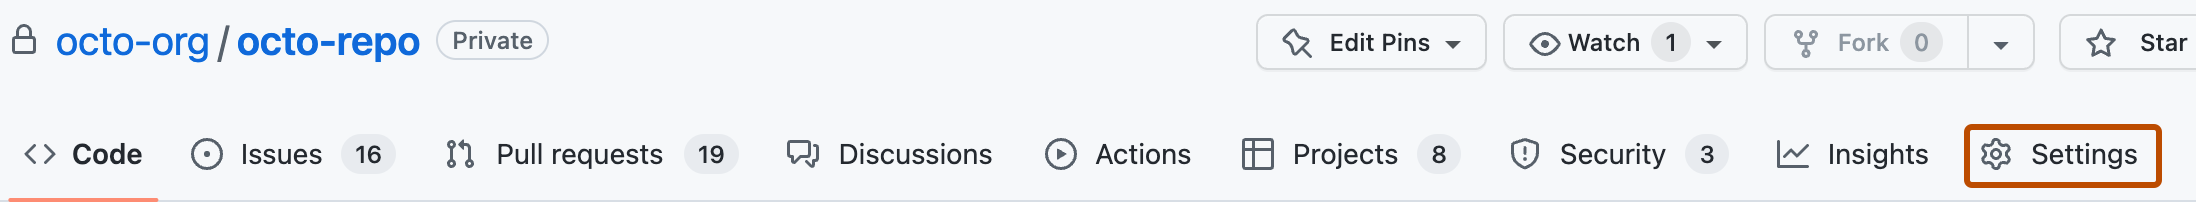
\includegraphics[width=\textwidth]{screenshots/gh-settings-tab.png}
    \caption{Repository navigation bar with the \textbf{Settings} tab highlighted \citep{ghConfigureDependabotAlerts}.}
    \label{fig:gh-settings-tab}
  \end{figure}

  \item In the \textbf{Security} section of the sidebar, click \textbf{Advanced Security}.

  \item Under \textbf{Dependabot alerts}, click \textbf{Enable} (or confirm the status is
    already enabled). Figure~\ref{fig:gh-dependabot-alerts-enabled} shows the
    \textbf{Disable} button, indicating that Dependabot alerts are currently enabled.

  \begin{figure}[H]
    \centering
    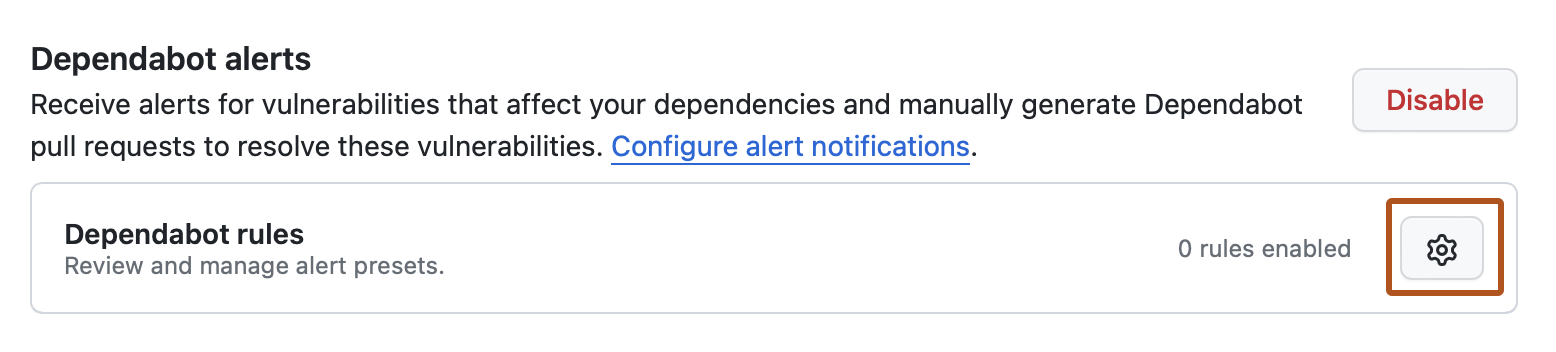
\includegraphics[width=\textwidth]{screenshots/gh-dependabot-alerts-enabled.png}
    \caption{Dependabot alerts enabled in \textbf{Advanced Security} settings \citep{ghPresetRulesDependabot}.}
    \label{fig:gh-dependabot-alerts-enabled}
  \end{figure}

  \item (Recommended) Enable \textbf{Dependabot security updates} so that GitHub can
    automatically propose remediation via pull requests when alerts are raised. When
    available, the alert details page provides a \textbf{Create Dependabot security update}
    action (Figure~\ref{fig:gh-create-security-update}).

  \begin{figure}[H]
    \centering
    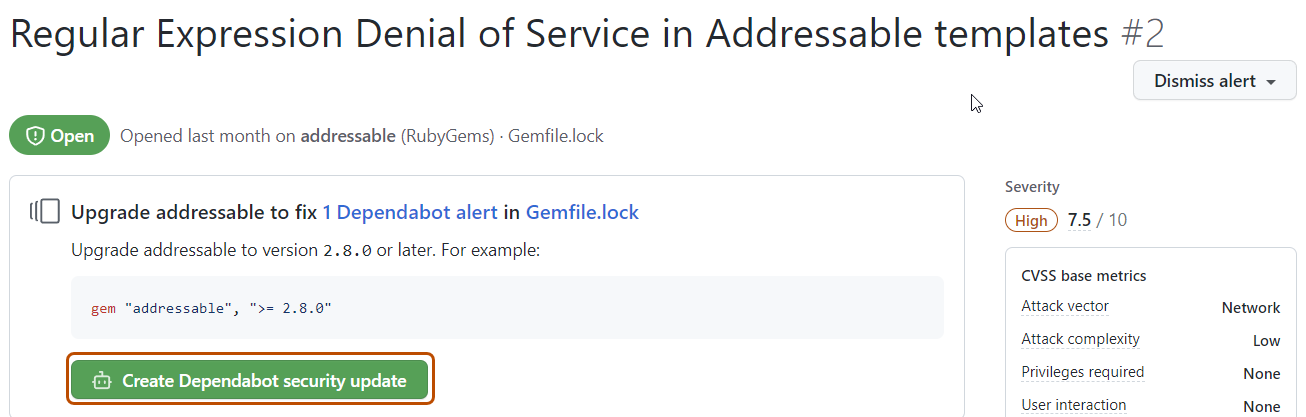
\includegraphics[width=\textwidth]{screenshots/gh-create-security-update.png}
    \caption{Dependabot alert details with the \textbf{Create Dependabot security update} button \citep{ghViewDependabotAlerts}.}
    \label{fig:gh-create-security-update}
  \end{figure}

  \item View alerts by navigating to the repository's \textbf{Security and quality} tab,
    then selecting \textbf{Dependabot} $\to$ \textbf{Vulnerabilities}. Figure~\ref{fig:gh-dependabot-alerts-list}
    shows a typical list of alerts with severity labels.

  \begin{figure}[H]
    \centering
    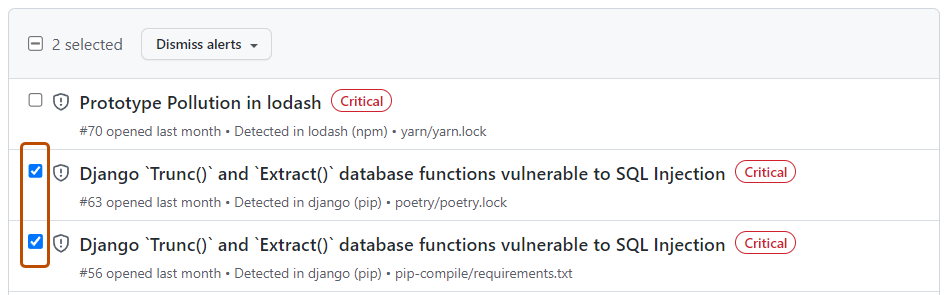
\includegraphics[width=\textwidth]{screenshots/gh-dependabot-alerts-list.png}
    \caption{Example Dependabot alerts list with severity labels \citep{ghViewDependabotAlerts}.}
    \label{fig:gh-dependabot-alerts-list}
  \end{figure}
\end{enumerate}

\subsubsection*{Interpreting Dependabot Alerts}

Each Dependabot alert presents:
\begin{itemize}
  \item \textbf{Package name and affected version(s)} --- identifies the vulnerable
    component and the version range with the flaw.
  \item \textbf{CVE identifier and CVSS severity score} --- contextualises the risk level
    (Low / Medium / High / Critical).
  \item \textbf{Patched version} --- the version that resolves the vulnerability.
  \item \textbf{Dependency path} --- whether the vulnerability is in a direct or
    transitive dependency, helping prioritise remediation effort.
  \item \textbf{Automated pull request} (if Dependabot security updates are enabled) ---
    a ready-made branch updating the manifest to the patched version.
\end{itemize}

This information allows development teams to triage, prioritise (critical CVEs first), and
remediate vulnerable dependencies with minimal manual research effort.

\subsection{How SCA Tools Contribute to Secure CI/CD Pipelines}

Software Composition Analysis tools integrate with CI/CD pipelines to provide automated,
continuous dependency security scanning throughout the development lifecycle
\citep{owaspDC}. Their contributions include:

\begin{itemize}
  \item \textbf{Shift Left enforcement.} By scanning dependencies at build time (e.g.,
    in a GitHub Actions \texttt{workflow.yml} step), SCA tools surface vulnerabilities
    before code merges to the main branch, preventing vulnerable components from
    reaching production.

  \item \textbf{Pipeline security gates.} SCA tools can be configured to \textit{fail
    the build} when dependencies with CVSS scores above a threshold (e.g., $\geq 7.0$
    High) are detected, enforcing a non-negotiable remediation requirement.

  \item \textbf{SBOM generation.} Tools such as Syft and OWASP Dependency-Track generate
    Software Bills of Materials, providing a complete inventory of all components in a
    release artefact \citep{ntia2021sbom}. SBOMs enable rapid impact analysis when new
    CVEs are disclosed.

  \item \textbf{Continuous monitoring.} Beyond build-time scanning, tools like
    Dependabot and Snyk continuously monitor dependency graphs against live vulnerability
    databases, generating alerts when new CVEs affecting already-deployed versions are
    published --- even between releases.

  \item \textbf{Licence compliance.} SCA tools also identify open-source licences,
    helping organisations avoid licence incompatibilities (e.g., GPL in a commercial
    product).
\end{itemize}

A representative GitHub Actions workflow step using OWASP Dependency-Check:

\begin{lstlisting}[caption={GitHub Actions SCA step using OWASP Dependency-Check}]
name: Security Scan
on: [push, pull_request]

jobs:
  dependency-check:
    runs-on: ubuntu-latest
    steps:
      - uses: actions/checkout@v4

      - name: Run OWASP Dependency-Check
        uses: dependency-check/Dependency-Check_Action@main
        with:
          project: 'paywave-digital'
          path: '.'
          format: 'HTML'
          args: >
            --failOnCVSS 7
            --enableRetired

      - name: Upload Dependency-Check Report
        uses: actions/upload-artifact@v4
        with:
          name: dependency-check-report
          path: ${{ github.workspace }}/reports
\end{lstlisting}

This pipeline step automatically fails any build introducing a dependency with a CVSS score
of 7 or higher, enforcing supply chain security as a mandatory quality gate consistent with
DevSecOps principles.

Dependabot's automated update behaviour is further controlled through a
\texttt{.github/dependabot.yml} configuration file committed to the repository. A
representative configuration for a Node.js project with GitHub Actions workflow monitoring
is shown below:

\begin{lstlisting}[caption={.github/dependabot.yml --- Scheduled Dependabot update configuration}]
version: 2
updates:
  - package-ecosystem: "npm"
    directory: "/"
    schedule:
      interval: "weekly"
    labels:
      - "security"
      - "dependencies"
    open-pull-requests-limit: 10

  - package-ecosystem: "github-actions"
    directory: "/"
    schedule:
      interval: "weekly"
\end{lstlisting}

This configuration instructs Dependabot to check both \texttt{npm} packages and GitHub
Actions workflow versions on a weekly schedule, automatically opening pull requests for
available updates. Integrating this file into the repository ensures dependency monitoring
is always active without requiring manual configuration through the GitHub UI.

\newpage

% ============================================================
% REFERENCES
% ============================================================
\bibliography{references}

\end{document}
